\subsection{Flood and landslide as discrete conditioning layers}
\label{subsec:results-flood}

The typical scenario in Porto Alegre reaches education in 9.4 minutes, food in 12.4 and health in 14.3, with F15 at 0.857, 0.728 and 0.673. Averaged across categories, the city reaches its services in 15.1 minutes, against 12.6 in Curitiba. The index G is 0.352 for education, 0.380 for food, 0.431 for health and 0.305 for transportation, and the dispersion is wider than in Curitiba. Among the cells that do reach a health facility, the slowest tenth takes more than 87.8 minutes, against 34.5. Transportation again departs from the pattern, with a mean of 24.0 minutes and F15 of 0.221, consistent with the sparse mapping of stops noted in Section~\ref{subsec:scope-comparison}.

The \texttt{flood} scenario raises the overall PTh from 15.1 to 20.7 minutes and lowers F15 from 0.620 to 0.510, with a median cell increase of 3.3 minutes and a 90th percentile of 46 minutes. No cell loses access, because the factor is finite and only multiplies the cost of the edge, leaving the graph connected. The magnitude far exceeds the thermal case because the factor is far larger. The three risk classes carry factors of 1.71, 1.86 and 2.14, applied to a flooded area of 250.8~km$^2$, which is 47.6\% of the municipality. Figure~\ref{fig:results-porto-alegre-flood} presents the resulting access times and the corresponding changes across cells.

\begin{figure}[htbp]
  \centering
  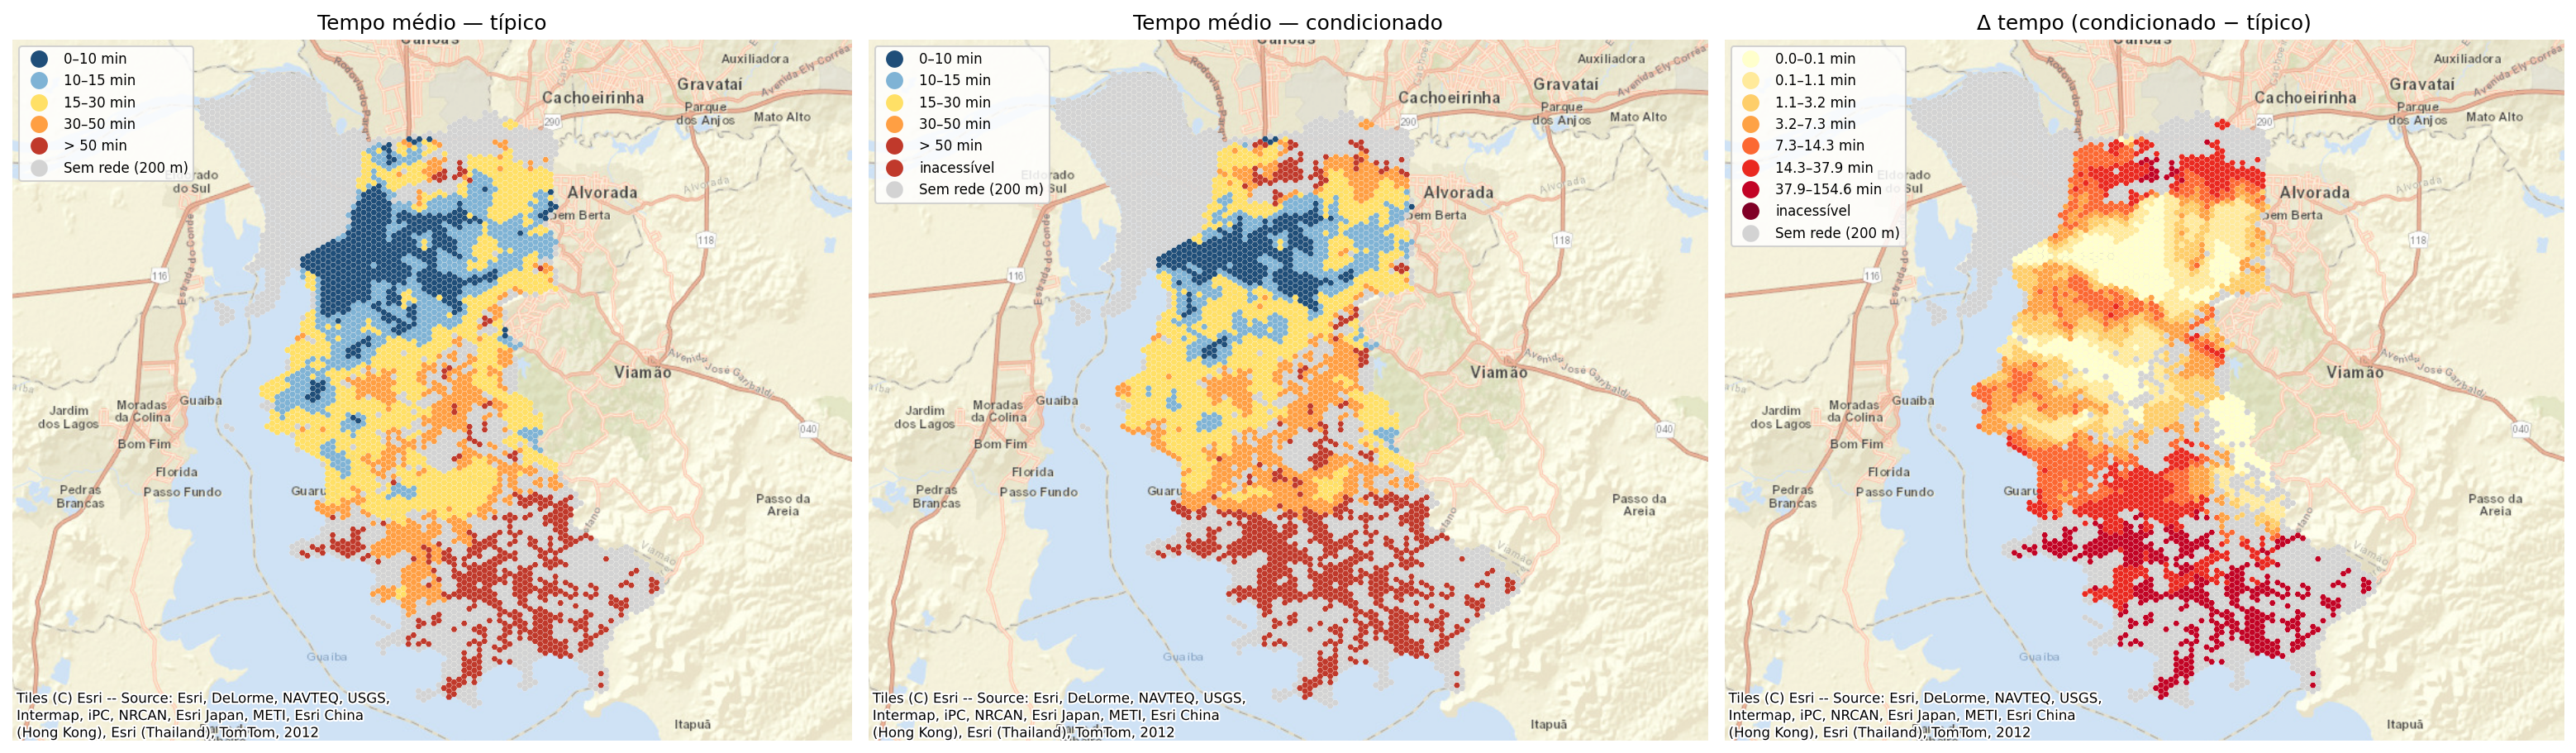
\includegraphics[width=1\textwidth]{figs/porto_alegre_inundacao.png}
  \caption{Porto Alegre under the \texttt{flood} scenario. Left: mean access time in the typical scenario. Centre: the same cells after the flood factor is applied. Right: the per-cell increase in access time, in minutes. The delay covers the floodplain and tapers towards the edges of the affected polygons; no cell loses network.}
  \label{fig:results-porto-alegre-flood}
\end{figure}

The \texttt{landslide} scenario removes 9{,}465 of the 36{,}780 cell--POI pairs from reach, or 25.7\% of the matrix, and leaves every other pair untouched. The median increase among the pairs that survive is zero, because a cell outside the mapped polygons keeps its original cost. An infinite factor therefore produces a different outcome from a finite one, and the framework reports it separately. In the figure, a cell inside the affected polygons either falls in a delay class or is drawn in red, the top of the scale, which marks loss of access; grey marks cells beyond the snapping threshold, which never enter the matrix. Figure~\ref{fig:results-porto-alegre} shows the two outcomes together.

\begin{figure}[htbp]
  \centering
  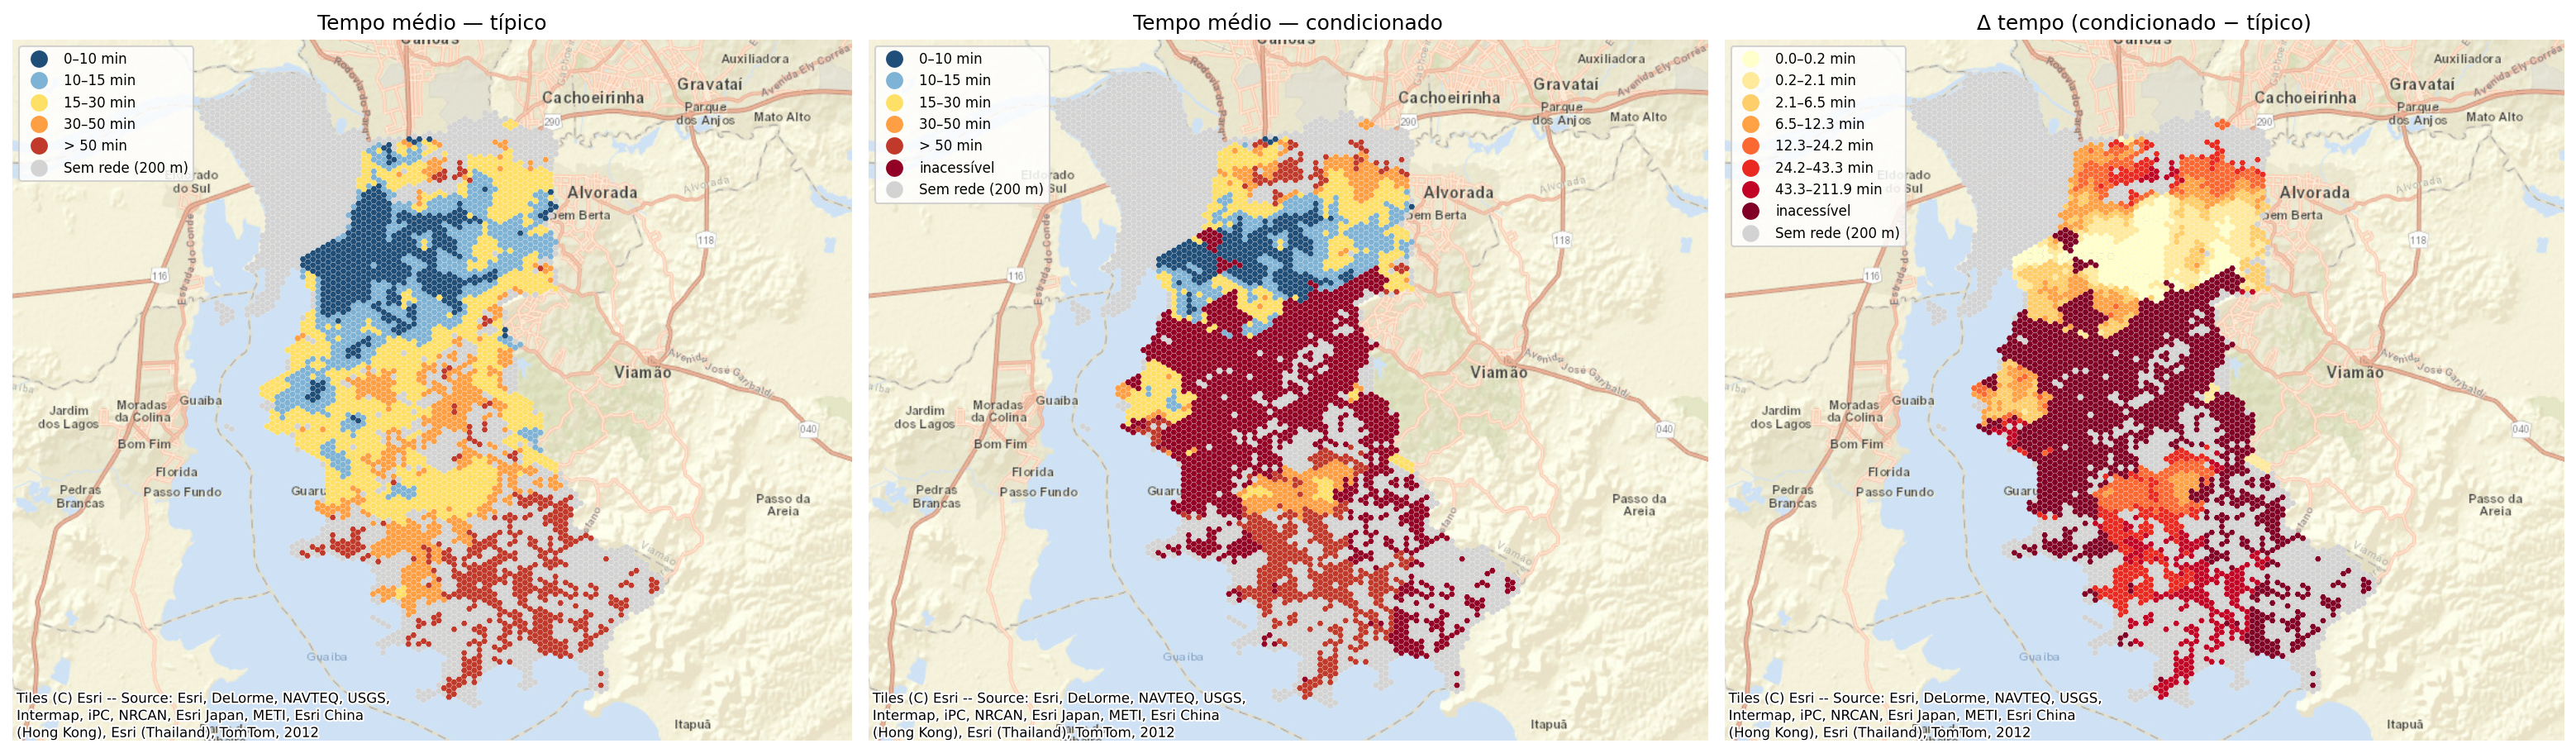
\includegraphics[width=1\textwidth]{figs/porto_alegre_combinado.png}
  \caption{Porto Alegre under the \texttt{flood+landslide} scenario. Left: mean access time in the typical scenario. Centre: the same cells after both layers are applied, with loss of access drawn in red at the top of the scale. Right: the per-cell increase in access time, in minutes. Grey marks cells beyond the snapping threshold, which carry no pedestrian network. The two hazards leave different marks, as flooding shades a broad area while landsliding removes whole cells from the reachable set.}
  \label{fig:results-porto-alegre}
\end{figure}
